% !TEX encoding = UTF-8
% !TEX TS-program = pdflatex
% !TEX root = ../main.tex
% !TEX spellcheck = en-GB

\documentclass[final, 11pt, a4paper, titlepage, dvipsnames]{article}
\makeatletter
\AtBeginDocument{\let\hl\@firstofone}
\makeatother

\usepackage[english]{babel}
\usepackage[utf8]{inputenc}
\usepackage[hidelinks]{hyperref}
\usepackage{graphicx}
\usepackage{textcomp}
\usepackage{wallpaper}
\usepackage{color}
\usepackage{mathtools}
\usepackage{listings}
\usepackage{amssymb}
\usepackage[
	backend=biber,
	citestyle=numeric-comp,
	hyperref,
	backref,
	sorting=none
]{biblatex}

\graphicspath{{images/}}

\addbibresource{bibliography.bib}


\defbibheading{bibliography}
{
    \phantomsection 
    \addcontentsline{toc}{section}{\bibname}
    \section*{\bibname\markboth{\bibname}{\bibname}}
}

\setlength\bibitemsep{1.5\itemsep} 

%\DeclareBibliographyCategory{sampleCategory}

%\addtocategory{sampleCategory}{referenceID}

\definecolor{codegreen}{rgb}{0,0.6,0}
\definecolor{codegray}{rgb}{0.5,0.5,0.5}
\definecolor{backcolor}{rgb}{0.98,0.98,0.98}
\colorlet{punct}{red!60!black}
\definecolor{delim}{RGB}{20,105,176}

\lstset{
	backgroundcolor=\color{backcolor},
	commentstyle=\color{Peach}\ttfamily,
	keywordstyle=\color{RoyalBlue},
	numberstyle=\tiny\color{codegray},
	stringstyle=\color{SeaGreen}\ttfamily,
	basicstyle=\footnotesize\ttfamily,
	breakatwhitespace=false,
	breaklines=true,
	captionpos=b,
	keepspaces=true,
	numbers=left,
	numbersep=5pt,
	showspaces=false,
	showstringspaces=false,
	showtabs=false,
	tabsize=2,
	frame=trbl, % draw a frame at the top, right, left and bottom of the listing
	frameround=ftff, % angolo in basso a destro curvo
	framesep=4pt, % quarter circle size of the round corners,
	inputencoding=utf8,
	extendedchars=true,
	literate={á}{{\'a}}1 {à}{{\`a}}1 {é}{{\'e}}1 {è}{{\`e}}1 {ù}{{\`u}}1 {ò}{{\`o}}1 {ì}{{\`i}}1,
	belowskip=1em,
	aboveskip=1em,
}

\lstdefinelanguage{XML}{
	% list of keywords
	morekeywords={application, uses-permission, uses, permission, xml, version, encoding, service, activity, intent -filter, manifest, fragment, LinearLayout, FrameLayout,
		application, service},
	morecomment=[s]{<!--}{-->}, % s is for start and end delimiter
	morestring=[b]" % defines that strings are enclosed in double quotes
}

\lstdefinelanguage{Java}{
	morekeywords={ListView, ArrayAdapter, Context, R, String, WifiManager, Intent,
		String, public, private, List, while, null, if, return, Cursor, Fragment, Uri,
		static, final, int, case, break, CursorLoader, ContentValues, HeadlessFragment,
		protected, @Override, boolean, TextView, switch, SharedPreferences, void,
		View, for, extends, class, FragmentTransaction, WorkoutDetailFragment, long,
		throw, new, this, true, false, Button},
	morecomment=[l]{//},
	morecomment=[s]{/*}{*/},
	morestring=[b]"
}

\lstdefinelanguage{json}{
	basicstyle=\normalfont\ttfamily,
	numbers=left,
	numberstyle=\scriptsize,
	stepnumber=1,
	numbersep=8pt,
	showstringspaces=false,
	breaklines=true,
	frame=lines,
	comment=[l]{//},
	keywords=[2]{id, title, message},
	keywordstyle=[2]{\color{RoyalBlue}},
	keywords=[3]{Array, String, Number, Date, ObjectId},
	keywordstyle=[3]{\color{Black}},
	literate=
	*{:}{{{\color{punct}{:}}}}{1}
	{,}{{{\color{punct}{,}}}}{1}
	{\{}{{{\color{delim}{\{}}}}{1}
	{\}}{{{\color{delim}{\}}}}}{1}
	{[}{{{\color{delim}{[}}}}{1}
	{]}{{{\color{delim}{]}}}}{1},
}

\newcommand{\university}{Università degli Studi di Padova}
\newcommand{\dept}{Department of Mathematics}
\newcommand{\faculty}{Master Degree in Computer Science}
\newcommand{\myyear}{Academic Year 2016/17}
\renewcommand{\title}{QuizFight}
\newcommand{\subtitle}{An Android trivia quiz application}
\newcommand{\fstauthor}{Alex Beccaro - 1156235}
\newcommand{\sndauthor}{Emanuele Carraro - 1155105}
\newcommand{\trdauthor}{Matteo Di Pirro - 1154231}

\begin{document}
	\begin{titlepage}
\begin{center}

\begin{LARGE}
\textbf{\university}\\
\end{LARGE}

\vspace{10pt}

\begin{Large}
\textsc{\dept}\\
\end{Large}

\vspace{10pt}

\begin{large}
\textsc{\faculty}\\
\end{large}

\vspace{30pt}
\begin{figure}[htbp]
\begin{center}

\includegraphics[height=6cm]{images/logo_unipd}
\end{center}
\end{figure}
\vspace{30pt} 

\begin{LARGE}
\begin{center}
\textbf{\title}\\
\end{center}
\end{LARGE}

\begin{Large}
	\begin{center}
		\textbf{\subtitle}\\
	\end{center}
\end{Large}

\vspace{20pt} 

\begin{large}
\begin{flushright}
\textit{\fstauthor \\ \sndauthor \\ \trdauthor}
\end{flushright}
\end{large}

\vspace{40pt}

\line(1, 0){338} \\
\begin{normalsize}
\textsc{\myyear}
\end{normalsize}

\end{center}
\end{titlepage} 
	\tableofcontents
	\newpage
	\section{Introduction}

The benefits of a gaming approach for learning are well-known. In fact,
people learn better and more when they play games. We are never tired of
playing.
After all, games mean fun. And fun means that our minds are relaxed and open
for gaining new knowledge.
This is why, over the last few years, scientists have begun to commission
more and more scientific games.
The goal is to involve people in science and let them learn new things.

Furthermore, nowadays there are many game shows that let people test their
trivia knowledge.
They are fun and useful because they allow both competitors and audience to
learn new things, while playing.
We develop QuizFight, a trivia quiz application allowing users to test their
trivia knowledge.
Contrariwise to popular game shows, we cannot reward users with money.
Instead they gain experience. 

The basic flow is simple. We identify a set of 20 topics and users can
dare each other with duels in three different topics.
Users can also choose to generate random topics for a duel.
Hence, a duel comprises of three different rounds each of which comprises
of five questions.
Each question has an associate difficulty level determining its score.
Difficulty levels range in [1, 3].
There are almost 1000 different questions available.

QuizFight ``programmatic'' goal is, on the other hand, to test how easily an
Android application can interact with different well-known service providers,
such as Google Play Services and Facebook.

We found that using their services is pretty simple, even if the learning curve
is not so linear.

In this paper we explain some QuizFight features and how they are
implemented.
We also discuss some current limitations and provide likely directions for
future work. 

The rest of this paper is organized as follows. Section~\ref{ref:design} explains
some design details. Section~\ref{sec:server} describes the choices we made for
QuizFight's server and how the Android application interacts with it. 
Section~\ref{sec:fcm} is about how notifications are sent to the clients.
Sections~\ref{sec:fb} and \ref{sec:ggames} illustrate how our application
interacts with both Facebook and Google for providing a consistent user
experience. Sections~\ref{sec:issues} describes some known issues due 
our use of Google Games. Our work is then concluded in Section~\ref{sec:limitations},
where we provide some lines for further work.
	
	\section{Application design}\label{ref:design}

QuizFight information model is depicted in Figure \ref{fig:quizfighter}.
The main entry point is \texttt{SignInActivity}.
Our game, in its very first version, requires the user to sign in with Google
Games. Hence, \texttt{SignInActivity} simply shows a button for the sign in.
The user's dashboard is \texttt{HomeActivity}.
Here the player can see their previous duels, both the completed and the
pending ones.
By tapping on a duel, a complete report of the result is shown.
When the duel has not been completed and when a new round is actually
available (i.e. when both the player and their opponent completed the
previous round), a button asking the user for answering the next questions
is shown.
Since showing every duel would incur in a bad user experience we show
only a limited number. We then provide a way to see the complete lists.

\begin{figure}[t]
	\centering
	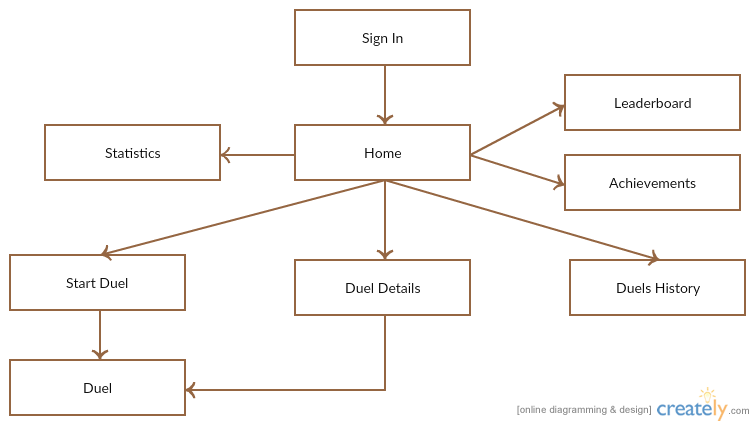
\includegraphics[width=0.9\linewidth]{QuizFightER}
	\caption{QuizFight information model}
	\label{fig:quizfighter}
\end{figure}

From \texttt{HomeActivity} a user can also see their current situation in terms
of ranks and achievements.
That information is directly retrieved and shown using Google's services.
In addition, QuizFight offers the possibility to take a look at a user's
statistics, such as the number of duels (or rounds) won versus the number of
duels (or rounds) played and the correct answers.
All these statistics are presented in bar charts.
Finally, there is the possibility to sign in with Facebook, for daring the
user's friends.

By tapping on the fight button it is possible to start a new duel.
Here, the adversary can be chosen in three different modalities:

\begin{itemize}
	\item \textbf{random};
	\item selected from the \textbf{leaderboard};
	\item selected from the \textbf{Facebook's friends list}.
\end{itemize}

After \texttt{DuelActivity} is shown, the user is able to answer the
questions of the round. At the round's ending a dialog is shown to notify 
the user about their actual round's score. If both the player and the opponent 
have terminated the current round they are both notified about a new round 
available (if any), or about the duel's ending (with the final score). 

	\section{QuizFight server}

QuizFight relies on a Node.js server and a MongoDB database.
We choose these technologies consequently to the choice of the JSON format for
exchanging data.
In fact, since Node.js uses JavaScript as a language, it is well suited for
dealing with JSON messages.
The same motivation applies for MongoDB. It is a NoSQL database, where
documents can be thought as JSON files.
The flexibility of both communication and saving convinced us to use this
stack.
Furthermore there are no strong evidences, based on performance and overhead,
against the use of a Node.js server rather that a Java one. 

To interact with the database we use a well-known Node.js's package:
\texttt{mongoose.js}.
By following the Model-View-Controller design pattern we define both
models and controllers server side and let the clients provide the View-part.

For exposing our APIs, we use \texttt{Express.js}.
Each API is represented by a \texttt{Route} object.
No access is directly made from the routes to the model objects.
Instead, they use some methods provided by the controllers, exactly as stated
by the MVC pattern.

The server is a fundamental component in QuizFight. In fact, it is used to
store the data of the users and duels, and it also performs the binding
$<$player, opponent$>$ and keeps the actual questions.
Duels are thus generated server side and sent, on demand, to the clients,
round by round.

Users identification is based on their GGames usernames.
This provides an effective way to retrieve their information and to bind
them in duels.
We could have used MongoDB identifiers, instead we used usernames for their
simplicity.
In fact, using MongoDB's ids would have required too much effort.
Clients are unaware of how the server identifies users, so in this case the
best we could do client side is to send usernames.
Then, on the server, for each operation involving users we should have
retrieved user's information.
This pattern, although possible, rapidly deteriorates to a lot of unnecessary
requests.
We then prefer using usernames, which we know by Google's assurance to be
unique.

\subsection{Client-server communication}
For communicating with the server we chose the Retrofit library. It is a 
type-safe REST client for Android (or just Java) developed by Square. 
It provides a powerful framework for interacting with APIs and sending 
network requests with the HTTP client \texttt{OkHttp}. Its request/response
API is designed with fluent builders and immutability. It supports both 
synchronous blocking calls and async calls with callbacks. 

This library makes downloading JSON or XML data from a web API fairly 
straightforward. Once the data is downloaded then it is parsed into a 
Plain Old Java Object (POJO) which must be defined for each ``resource'' 
in the response.

The communication obviously requires the \texttt{android.permission.INTERNET}
permission. We share only JSON objects. As aforementioned, our server is 
specifically designed for being efficient in JSON handling. Even if a 
communication paradigm based on XML would be more secure (as XML has a schema
defining exactly how the document should be), the JSON alternative is simpler 
and faster. Furthermore, we do not need an absolute confidence in the document. If
one or more required fields are missing, the server notifies the client using an
error response.

Using JSON arises a problem at client side. Java is a strongly typed language, so we
cannot freely manipulate objects as in JavaScript. We need a way to cast a JSON 
object into a Java (POJO) one. We do that using Gson, a Google's library for 
serializing and deserializing JSON objects. 

Following the object-oriented programming paradigm we design a scalable and easily 
manageable architecture for REST calls. Figure~\ref{fig:retrofit} shows a partial
class diagram for that. Only two concrete API calls are shown; for the others it 
is exactly the same.
\begin{figure}[h]
	\centering
	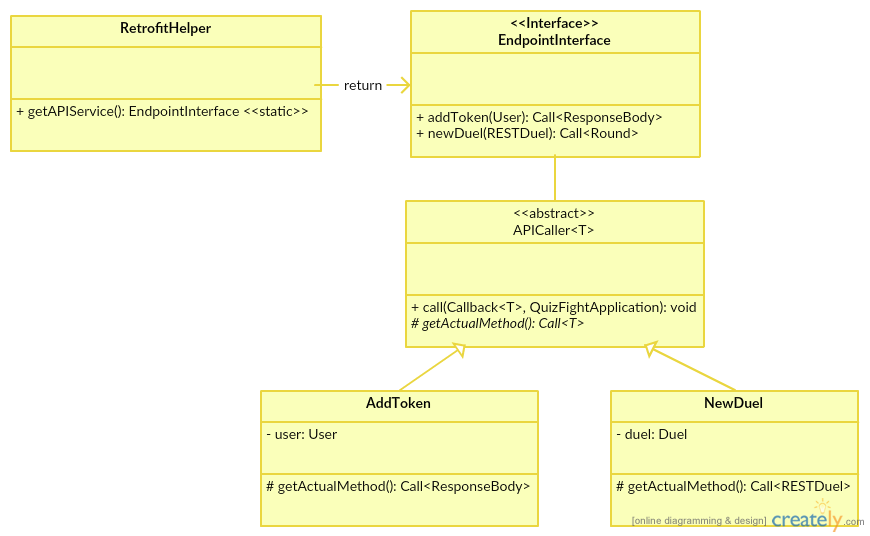
\includegraphics[width=0.9\linewidth]{Retrofit}
	\caption{High-level class diagram for API calls}
	\label{fig:retrofit}
\end{figure}

\texttt{RetrofitHelper} is the actual entry point. Its method \texttt{getAPIService()}
configures every parameter required, such as the base URL, the timeout, and the 
library for dealing with JSON. Then, via reflection, it creates on the fly a 
concrete \texttt{EndpointInterface} instance. The latter actually contains the
methods corresponding to the API calls. Retrofit allows us to specify HTTP
parameters by using Java-based annotations, such as \texttt{@Headers} for the
headers, and \texttt{@PUT("endpoint")} for a PUT call. 

Those methods return a generic \texttt{Call<T>} object. The type parameter 
represents the POJO object returned by the server. In this sense Retrofit is a
type-safe REST library. The \texttt{EndpointInterface} concrete instance is then
used by an abstract class, \texttt{APICaller}, which basically implements a mix
of the template method and command design patterns. Each concrete class extending
\texttt{APICall} should have a field representing the object to be sent, 
as a parameter, to the server. Then it implements the abstract method 
\texttt{getActualMethod()} in order to make the right call with the right 
parameters. It is invoked by the \texttt{APICall}'s \texttt{call()} method,
which also enqueues the actual execution to be performed in an asynchronous way. 

Then, whenever a Java class wishes to communicate with the server, it must 
instantiate the corresponding API class, give a parameter to it and provide
two callbacks, \texttt{onResponse()} and \texttt{onFailure()}, for handling the
corresponding situations. Listing~\ref{lst:servercall} shows an example.

\begin{lstlisting}[language=Java, caption={Server call example}, label={lst:servercall}]
new AddToken(new User(
	Games.Players.getCurrentPlayer(client).getDisplayName(),
	token,
	Secure.getString(getContentResolver(), Secure.ANDROID_ID)
)).call(new Callback<ResponseBody>() {
	@Override
	public void onResponse(Call<ResponseBody> call, Response<ResponseBody> response) {}
	
	@Override
	public void onFailure(Call<ResponseBody> call, Throwable t) {}
}, getApplication());
\end{lstlisting}
	\section{Firebase Cloud Messaging}

Duels are interactive by definition. A user \texttt{A} can dare another user
\texttt{B} at any time as well as \texttt{B} can complete a round at an
 time.
An application forcing the users to manually check for updates (the so
called \textit{polling}) would probably occur in a bad user experience.

A smarter approach is the so-called \textit{push notification}.
Our server sends out different messages for different situations.
Clients (i.e. the app's instances) need only to be listening for news.
The users are notified about new duel dares, new rounds available and duels
completion. Tapping on those notification result, of course, in QuizFight
opening the appropriate Activity.

A key issue is actually how to implement from scratch this protocol.
Some challenges would be the following:

\begin{itemize}
	\item How many times per second should the app check for updates?
	\item How should we identify a particular installation?
	\item How should we deal with new installations on different user's devices?
\end{itemize}

We then rely on a third-party well-known messaging protocol completely
integrated with Google: \textbf{Firebase Cloud Messaging} (FCM from now on).
It is a cross-platform messaging solution that lets us reliably deliver
messages at no cost.
Using FCM, we notify a client app that something is available to sync.
Its architecture is based on the following two main components:

\begin{itemize}
	\item A trusted environment such as an app server on which to build,
target and send messages, and
	\item An iOS, Android, or Web (JavaScript) client app that receives
messages.
\end{itemize}

FCM basically allows server implementations to send out messages to single
devices, groups or by topic.

QuizFight uses only the former, since is simple and well suited for its
purposes. This mode relies on installation tokens. At the very first
installation a token is generated.
This token is unique, but it may vary through the device's life.
In fact, if the user reinstalls the app or if they performs a cache wipe,
the token changes.
This is why both at client and server side a mechanism is required to
manage the token's life cycle.
Furthermore, different instances of the same app in different user's devices
have different tokens associated to them.
Hence, a notification has to be sent out to every different device, and
different tokens have to be managed server side.

\subsection{Client side}
FCM requires two services running on the target device.
They are used to check for token updates (remember a token is different after
a cache wipe) and to be listening for new messages.
Their declaration in the manifest is shown in Listing~\ref{lst:fcmservices}.

\begin{lstlisting}[language=xml, caption={FCM Services}, label={lst:fcmservices}]
<service android:name=".services.CustomFirebaseInstanceID">
	<intent-filter>
		<action android:name="com.google.firebase.INSTANCE_ID_EVENT"/>
	</intent-filter>
</service>
<service android:name=".services.MessagingService">
	<intent-filter>
		<action android:name="com.google.firebase.MESSAGING_EVENT"/>
	</intent-filter>
</service>
\end{lstlisting}

\texttt{CustomFirebaseInstanceID} basically monitors the token.
As said, the registration token may change when:

\begin{itemize}
	\item the app is restored on a new device;
	\item the user uninstalls/reinstalls the app;
	\item the user clears app data.
\end{itemize}

This service extends \texttt{FirebaseInstanceIdService} and overrides the
method \texttt{onTokenRefresh()}.
When a new token is available, it is sent to the server.
QuizFight also sends \texttt{Settings.Secure.ANDROID\_ID}, in order to
maintain the binding $<$device, token$>$. Even though the use of this field is
discouraged for most use cases, here it is necessary because we need to have
the strong guarantee that a token must correspond to one device.
Below are more details about that. \\

\texttt{MessagingService} is used for receiving new messages and extends 

\texttt{FirebaseMessagingService}. FCM provides two different message types:
\textbf{notification} and \textbf{data}.
The former can be sometimes thought of as ``display message''.
FCM automatically displays the message to end-user devices on behalf of the
client app.
Notification messages have a predefined set of user-visible keys and an
optional data payload of custom key-value pairs.
In this case, if the app is not in the foreground, FCM provides the message to
the system tray and no ``custom'' methods are invoked.

This is why we rely only on data messages, handling both parsing and user
notification by hand.
We define a format for our messages, with both mandatory and Activity-dependent
fields. Listing~\ref{lst:notification} shows the mandatory ones.

\begin{lstlisting}[language=json, caption={Mandatory fields for a notification}, label={lst:notification}]
{
	id: String,
	title: String,
	message: String
}
\end{lstlisting}

\texttt{id} is used to identify the notification type, and for opening the
appropriate Activity at ``tap time''.

\texttt{title} and \texttt{message} have the same meaning of the correspondent
fields used in Android's notifications.
Every \texttt{id} corresponds to a different triggered action, each of which
requires specific parameters agreed with the server.

Both \texttt{CustomFirebaseInstanceID} and \texttt{MessagingService} are
started services and they are not bound to any other component.
This is necessary because they have to live and be listening for updates,
both regarding token and new notifications.
They are started at the device boot, via a broadcast receiver: 
\texttt{QuizFightReceiver}, which is triggered by the \texttt{BOOT\_COMPLETED}
event.
They neither never stop themselves or are stopped by any other QuizFight
component. 

\subsection{Server side}
QuizFight's server is responsible for sending out notifications to clients. As we said, each app's instance is identified by using a unique token which life-cycle is managed by FCM. Nonetheless, we have to provide a way to handle token changes and multiple tokens for the same user. Fortunately, FCS allows us to send out almost 1000 messages at a time. We believe a user will not use more than 1000 devices with our application, so we consider this as a safe bound.

Any time the token varies the client sends the new one to the server. It also sends \texttt{Settings.Secure.ANDROID\_ID}. Android discourages the use of such an identifier and recommends alternatives such as \textbf{Instance ID} or \textbf{globally unique ID} (GUID). Unfortunately those solutions are not suitable for our purposes. In fact, they provide a way to identify an application's \textit{instance}, but we already have something like that (i.e. FCM's tokens). Another solution could be the \textbf{Advertising IDs}, but they are user-resettable. This is why we had to rely on a non-resettable hardware identifier, such as \texttt{ANDROID\_ID}.

The client sends also the current logged user's username. Since users are identified using their Google Games' username, there is no other way to actually identify a user server-side. Then the server simply retrieves a document representing that user, looks for the actual device and substitutes the old token with the new one. In this way as soon as the token varies the server is notified by \texttt{CustomFirebaseInstanceID} and keeps everything up to date. Of course, if no device with the actual \texttt{ANDROID\_ID} is found, a new device is added with the new token. From then on the new device will receive every notification.

When the server has to send out a new message it looks up users by their Google Games' username. It retrieves every device and every token (which is up to date by construction) and mails both the mandatory fields and the situation-dependent payload. We developed a module, \texttt{sendMessage}, which performs lookups and sending. Every message's information is directly provided by the REST service itself, so it is entirely a decentralized architecture without any dependency between the sending module and the information to be sent out.



	\section{Facebook login}\label{sec:fb}

In QuizFight, a user can challenge her friends on Facebook.
Although we could have let a user to search an adversary among her Google
contacts, we preferred to give her the possibility to log in with Facebook.
This decision is based on the observation that probably a person has more
friends on Facebook than contacts on Google.

In \texttt{HomeActivity}, a user can log in with Facebook and then, in

\texttt{StartDuelActivity} she can take a look at the list of
Facebook friends and choose one as adversary. \\

QuizFight requires the user\_friends permission in order to display the
list of a user's Facebook friends.

When a user log in with Facebook, her Facebook id is sent to the server and
saved to the correspondent user entry.

Then, when a user challenge a Facebook friend, the Facebook id of the friend
is retrieved and used to find the correspondent GGame username.
Finally, the duel can start.

	\section{Google Games}
Google Play Games (GGames from now on) provides a way to easily manage every detail of a game. By using it, users may complete achievements and quests, see ranks and experience a consistent feeling thorough difference devices. At the administrator side, it allows us to configure everything by using the Google Play Console.

We use GGames for a number of purposes. First of all, since QuizFight is a game, we define different achievements with an increasing difficulty level. Examples are ''\textit{Win 100 duels}'', ''\textit{Answer correctly to 1000 questions}'' or ''\textit{Score 45 points in a duel}''. As usual, by unlocking achievements the users gain experience. We also collect information about different events, such as the number of correct answers, the number of duels, or rounds, played and so on. Using GGames for storing those statistics is useful because it provides a very easy interface and allows us not to reinvent the wheel by reimplementing everything from scratch. The most important service we used is \textbf{Saved Games}, as discussed below.

\subsection{Sign In}

\subsection{Saved Games}
The most important service used in QuizFight is named \textbf{Saved Games}. It gives us a convenient way to save our players' game progression to Google's servers. We can then retrieve the saved game data to allow returning players to continue a game at their last save point from any device. The Saved Games service makes it possible to synchronize a player's game data across multiple devices. For example, if you have a game that runs on Android, you can use the Saved Games service to allow a player to start a game on their Android phone, and then continue playing on a tablet without losing any of their progress. Even if we save anyway the data on our server's database, Saved Games allows us to limit the network traffic with the server and provides an easy way to store the information even if the device has no connectivity. In fact, if the device is disconnected, Saved Games stores locally the data to be saved and, at the very first reconnection, it sends that to Google's servers.

A saved game consists of two parts:
\begin{itemize}
	\item an unstructured binary blob: this data can represent whatever we choose, and our game is responsible for parsing and writing to it;
	\item structured metadata: additional properties associated with the binary data that allow GGames services to visually present Saved Games in the default Saved Games list user interface (UI), and to present useful information in the GGames app (for example, last updated timestamp).
\end{itemize}
A game can write an arbitrary number of Saved Games for a single player, subject to user quota, so there is no hard requirement to restrict players to a single save file. Every game may save up to 3MB blobs. They are stored in the player's Google Drive space. Google ensures read/write isolation: only QuizFight is able to read QuizFight's saved data.

Figure~\ref{fig:saved-games-hierarchy} shows how we interact with Saved Games.
\begin{figure}
	\centering
	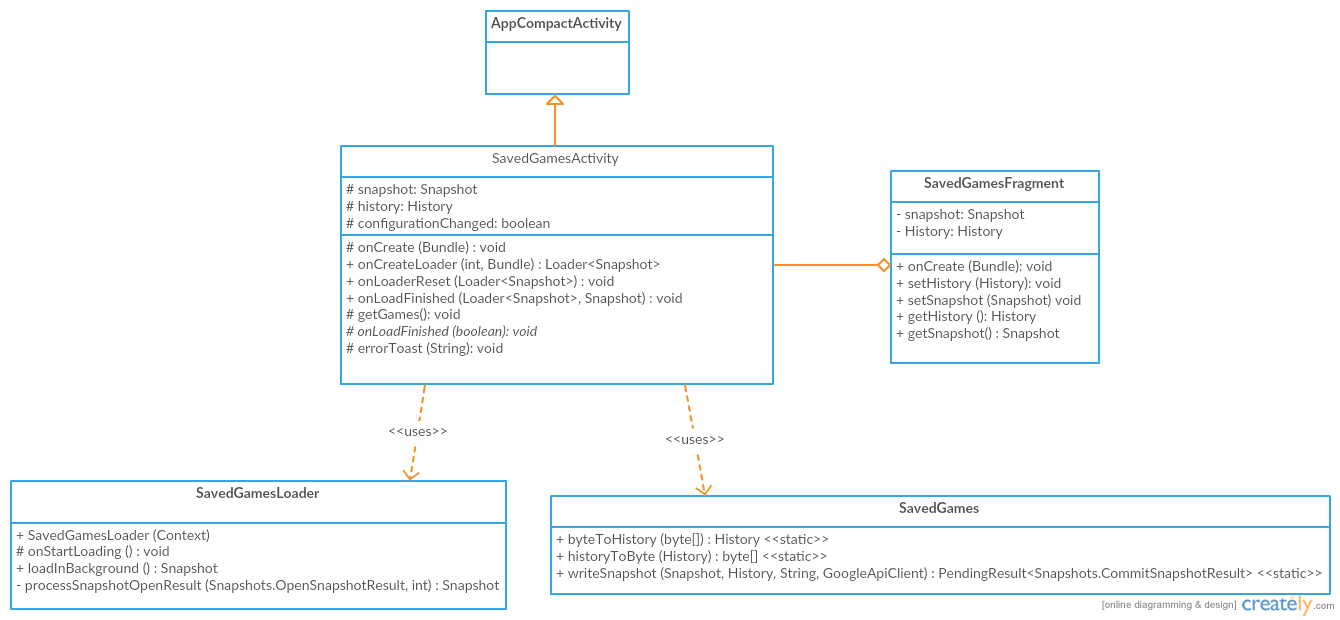
\includegraphics[width=1\linewidth]{SavedGamesHierarchy}
	\caption[Saved Games Hierarchy]
	\label{fig:saved-games-hierarchy}
\end{figure}

	
	%bibliography
	\newpage
	\nocite{*}
	\printbibliography 
	
\end{document}
